%%%%%%%%%%%%%%%%%%%%%%%%%%%%%%%%%%%%%%%%%
% Developer CV
% LaTeX Template
% Version 1.0 (28/1/19)
%
% This template originates from:
% http://www.LaTeXTemplates.com
%
% Authors:
% Jan Vorisek (jan@vorisek.me)
% Based on a template by Jan Küster (info@jankuester.com)
% Modified for LaTeX Templates by Vel (vel@LaTeXTemplates.com)
%
% License:
% The MIT License (see included LICENSE file)
%
%%%%%%%%%%%%%%%%%%%%%%%%%%%%%%%%%%%%%%%%%

%----------------------------------------------------------------------------------------
%	PACKAGES AND OTHER DOCUMENT CONFIGURATIONS
%----------------------------------------------------------------------------------------

\documentclass[9pt]{developercv} % Default font size, values from 8-12pt are recommended

%----------------------------------------------------------------------------------------

\begin{document}

%----------------------------------------------------------------------------------------
%	TITLE AND CONTACT INFORMATION
%----------------------------------------------------------------------------------------

\begin{minipage}[t]{0.525\textwidth} % 45% of the page width for name
	\vspace{-\baselineskip} % Required for vertically aligning minipages

	% If your name is very short, use just one of the lines below
	% If your name is very long, reduce the font size or make the minipage wider and reduce the others proportionately
	\colorbox{black}{{\HUGE\textcolor{white}{\textbf{\MakeUppercase{Felix}}}}} % First name

	\colorbox{black}{{\HUGE\textcolor{white}{\textbf{\MakeUppercase{Hoffmann}}}}} % Last name

	\vspace{6pt}

	{\huge Bachelorstudent Informatik} % Career or current job title

 	\vspace{0.5cm} % Required for vertically aligning minipages

	% The first parameter is the FontAwesome icon name, the second is the box size and the third is the text
	% Other icons can be found by referring to fontawesome.pdf (supplied with the template) and using the word after \fa in the command for the icon you want
	\icon{Asterisk}{10}{15.05.2000 in Berlin}\\
	\icon{MapMarker}{10}{Ernsthaldenstaße 43, 70565 Stuttgart}\\
	\icon{Phone}{10}{+49 176 2147 0118}\\
    \icon{At}{10}{\href{mailto:felix.hoffmann@hpe.com}{felix.hoffmann@hpe.com}}\\
	\icon{Github}{10}{\href{https://github.com/felixhoffmnn}{felixhoffmnn}}\\
\end{minipage}\hfill
\begin{minipage}[t]{0.375\textwidth} % 27.5% of the page width for the first row of icons
	\vspace{-\baselineskip} % Required for vertically aligning minipages

    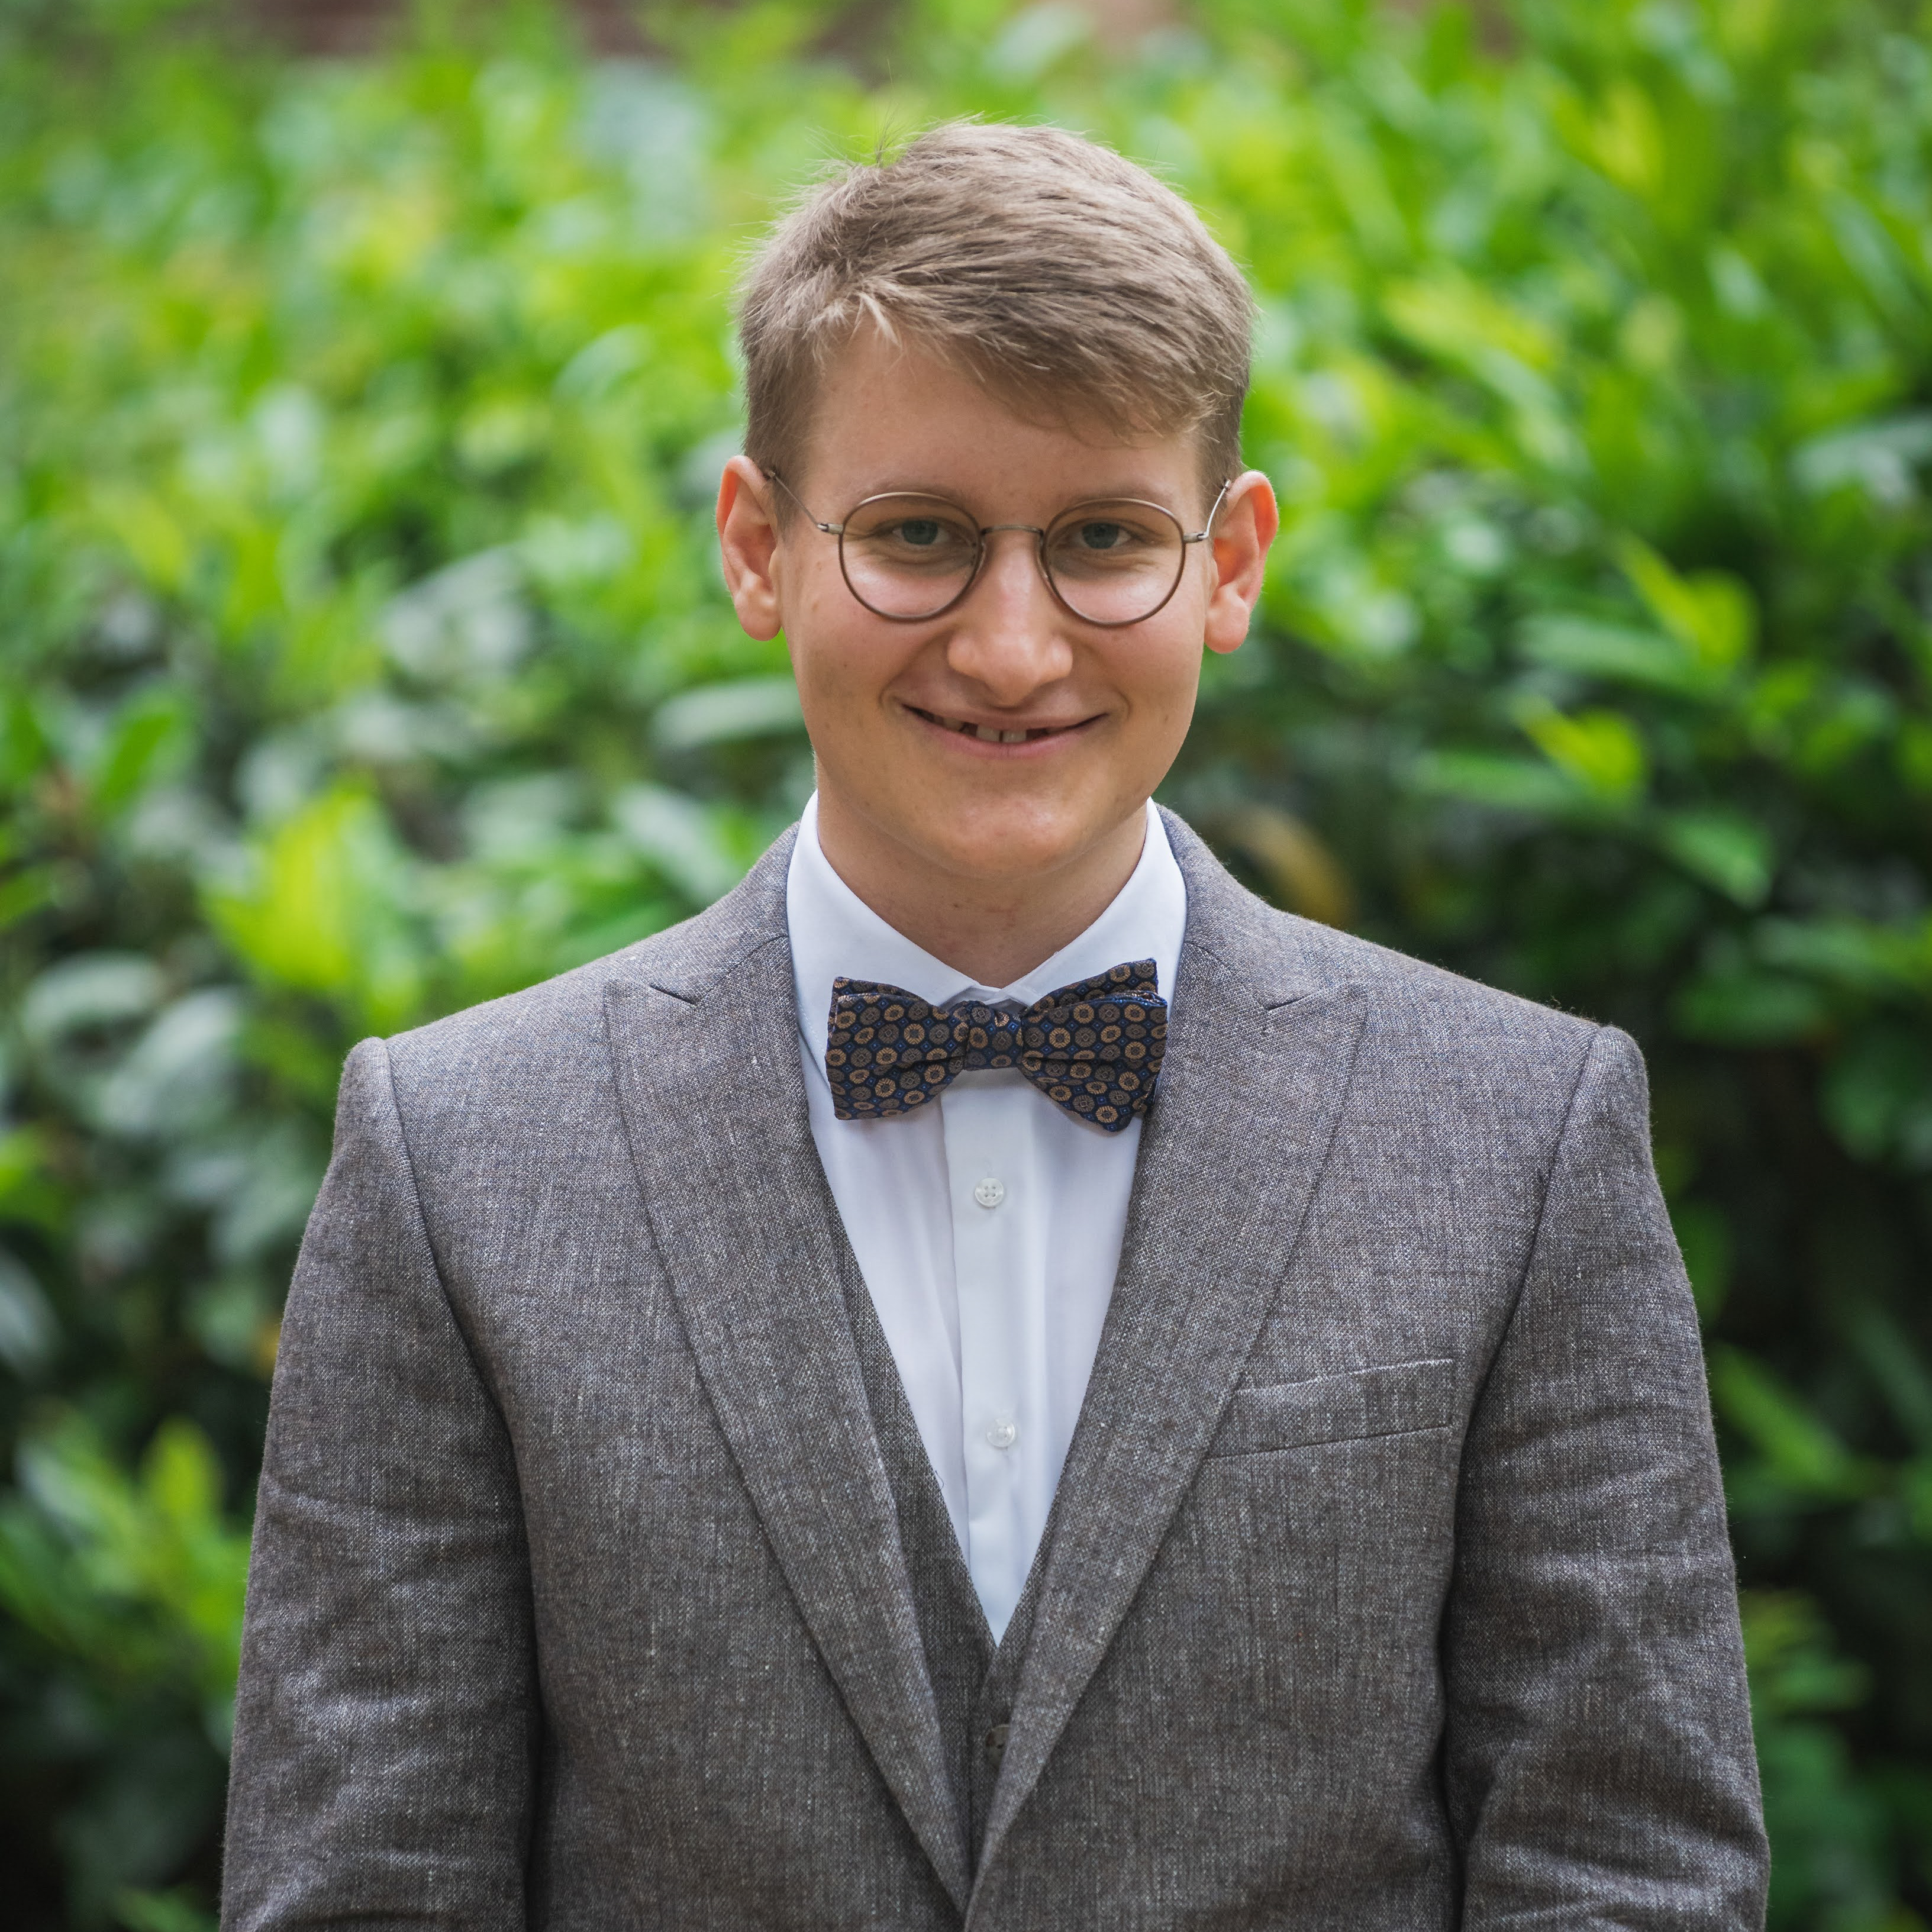
\includegraphics[width=\textwidth]{data/images/DSC02105-2.jpg}
\end{minipage}

\vspace{0.5cm}

%----------------------------------------------------------------------------------------
%	INTRODUCTION, SKILLS AND TECHNOLOGIES
%----------------------------------------------------------------------------------------

\cvsect{Ziele}

Schon seit meiner Schulzeit interessierte ich mich für aktuelle Technologien und wie man sie optimal einsetzen kann. Beispiele dafür sind mein Einsatz für digitales Arbeiten während meines Abiturs, aber auch aktuelle Projekte wie meine Studien- und Bachelorarbeit, als auch meine nebenberufliche Tätigkeit als Webentwickler.

\vspace{0.2cm}

Diese technischen Kenntnisse und Interessen möchte ich weiter mit einem Master im Bereich Data Engineering oder Software-Engineering vertiefen.

%----------------------------------------------------------------------------------------
%	INTRODUCTION, SKILLS AND TECHNOLOGIES
%----------------------------------------------------------------------------------------

\vspace{0.5cm}

\begin{minipage}[t]{0.45\textwidth}
	\vspace{-\baselineskip} % Required for vertically aligning minipages

	\cvsect{Engagement}

	Während des Abiturs war ich Klassensprecher und Mitglied im Schülerrat. Während meines Bachelorstudiums habe ich mich als Kurssprecher und Mitglied in der JAV eingebracht und organisatorische Fähigkeiten bewiesen.
\end{minipage}\hfill
\begin{minipage}[t]{0.45\textwidth}
	\vspace{-\baselineskip} % Required for vertically aligning minipages

	\cvsect{Skills}

	Python, TypeScript, React, SQL, Determined AI, Kubernetes, Java, UI- und UX-Design, Webentwicklung und Adobe XD

    \vspace{0.2cm}

    Anpassungsfähigkeit, Projektmanagement (SCRUM, Design Thinking) und kreatives Arbeiten
\end{minipage}

%----------------------------------------------------------------------------------------
%	EXPERIENCE
%----------------------------------------------------------------------------------------

\cvsect{Berufserfahrung}

\begin{entrylist}
	\entry
	{1/2023 -- 2/2023}
	{Front-end Optimierung}
	{Poinnext Services (HPE)}
	{Ladezeiten-Optimierung eines React-Frontends mittels Server-Side Pagination und Backend-Filtering.\\ \texttt{React}\slashsep\texttt{Typescript}\slashsep\texttt{Optimierung von Ladezeiten}}
	\entry
	{6/2022 -- 9/2022}
	{GPU Benchmarking}
	{Hewlett Packard Labs (HPE)}
	{Benchmarking von Algorithmen (z. B. Parameter Server und Ring All-Reduce) zum Trainieren von Machine Learning Modellen auf verteilten Systemen. Das Trainieren erfolgte auf der Maschine Learning Plattform „Determined AI“ mittels Kubernetes und Docker Containern. \\ \texttt{Determined AI}\slashsep\texttt{Kubernetes}\slashsep\texttt{Machine Learning}\slashsep\texttt{Python}}
	\entry
	{12/2021 -- 3/2022}
	{Front-end Development}
	{Digital Edge Ratingen (DXC)}
	{Umsetzung eines React Frontends zur 3D-Visualisierung von Diagrammen und Prozessen. State-managment erfolgte mittels Zustand und 3D Interaktion mittels React Three Fiber. \\ \texttt{React}\slashsep\texttt{Three.js}\slashsep\texttt{3D-Visualisierung}}
	\entry
	{3/2021 -- 5/2021}
	{No-Code/Low-Code Development}
	{Digital Service Innovation (DXC)}
	{Umsetzung einer zentralen Speicherlösung mittels einer Microsoft PowerApp. Interaktion anhand REST APIs mit Java Spring Backend. \\ \texttt{Power Apps}\slashsep\texttt{Knowledge Management}}
	\entry
	{10/2020 -- 11/2020}
	{Analyse von Monitoring-Tools}
	{Pointnext Services (HPE)}
	{Analyse von Open Source Monitoring Tools wie zum Beispiel Nagios und Zabbix. Die Erkenntnisse wurden in einer Tabelle und Projektarbeit dokumentiert. \\ \texttt{Monitoring}}
\end{entrylist}

\vspace{0.5cm}

\begin{entrylist}
	\entry
	{Seit 2021}
	{Nebenberufliche Tätigkeit als Webentwickler}
	{Felix Emmanuel}
	{Umsetzung von statischen Webseiten, Fotografie und technische Beratung (Link zur Webseite: \textit{\href{https://felixemmanuel.de}{felixemmanuel.de}}) \\ \texttt{Wordpress}\slashsep\texttt{Adobe XD}\slashsep\texttt{Fotografie}}
\end{entrylist}

%----------------------------------------------------------------------------------------
%	EDUCATION
%----------------------------------------------------------------------------------------

\cvsect{Ausbildung}

\begin{entrylist}
	\entry
	{2020 -- 2023}
	{Bachelor of Science}
	{DHBW Stuttgart \& HPE}
	{Duales Studium im Bereich Informatik\\ \texttt{Kurssprecher}\slashsep\texttt{Mitglied in der JAV}}
	\entry
	{2017 -- 2020}
	{Abitur}
	{Oberstufenzentrum Märkisch Oderland}
	{Abitur in 3 Jahren mit technischem Schwerpunkt (Maschinen- und Kommunikationstechnik)\\ \texttt{Gesamtnote: 1,6}\slashsep\texttt{Klassensprecher}\slashsep\texttt{Mitglied im Schülerrat}}
	\entry
	{2006 -- 2017}
	{Mittlerer Schulabschluss}
	{bundtStift Schulen}
	{Grundschule \& Gymnasium mit kreativem Schwerpunkt}
\end{entrylist}

%----------------------------------------------------------------------------------------
%	International experience
%----------------------------------------------------------------------------------------

\cvsect{Auslandserfahrung}

\begin{entrylist}
	\entry
	{2022}
	{Hewlett Packard Labs}
	{San Francisco, USA}
	{Auslandseinsatz im Network \& Distributed Systems Lab}
	\entry
	{2018}
	{Bildungs- und Begegnungsreise mit Workcamp}
	{Indien}
	{Reise für interkulturelle Zusammenführung und Hausbau-Workcamp als Hilfe für einen indigenen Stamm in Indien}
\end{entrylist}

%----------------------------------------------------------------------------------------
%	Projects
%----------------------------------------------------------------------------------------

\cvsect{Projekte}

\begin{entrylist}
  \entry
	{2023}
	{(Bachelorarbeit)}
	{DHBW Stuttgart \& Poinnext Services (HPE)}
	{Ladezeiten-Optimierung eines React-Frontends mittels adaptiven Backend-Filtering und gecachten Datensätzen.\\ \texttt{React}\slashsep\texttt{Typescript}\slashsep\texttt{Ladezeiten Optimierung}}
	\entry
	{2022 --  2023}
	{Studienarbeit}
	{DHBW Stuttgart}
	{NLP Projekt zur Erkennung von Parteien anhand von Tweets, Politischen Reden und Wahlprogrammen. Das trainierte Modell kann unter anderem zur Klassifikation Zeitungsartikeln eingesetzt werden.\\ \texttt{NLP}\slashsep\texttt{Python}\slashsep\texttt{Machine Learning}}
\end{entrylist}

%----------------------------------------------------------------------------------------
%	ADDITIONAL INFORMATION
%----------------------------------------------------------------------------------------

\begin{minipage}[t]{0.45\textwidth}
	\vspace{-\baselineskip} % Required for vertically aligning minipages

	\cvsect{Sprachen}

	\textbf{Deutsch} -- Muttersprache\\
	\textbf{Englisch} -- Verhandlungssicher\\
    \textbf{Französisch} -- Grundlagen\\
    \textbf{Spanisch} -- Grundlagen
\end{minipage}
\hfill
\begin{minipage}[t]{0.45\textwidth}
	\vspace{-\baselineskip} % Required for vertically aligning minipages

	\cvsect{Interessen}

	Volleyball, Fotografie und Webdesign
\end{minipage}

%----------------------------------------------------------------------------------------

\end{document}
